\documentclass{standalone}
\usepackage{tikz}
\usepackage{verbatim}
\usetikzlibrary{positioning}
\begin{document}
\pagestyle{empty}
  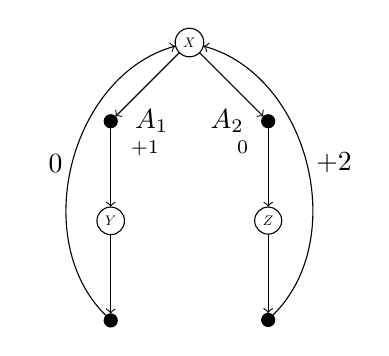
\begin{tikzpicture}
    \node[draw,circle,scale=1/2] (x) at (0, 0) {$X$};
    \node[draw,circle,fill,scale=1/2] (a1) at (-1, -1) {};
    \node[draw,circle,fill,scale=1/2] (a2) at ( 1, -1) {};
    \node[draw,circle,below=1cm of a1,scale=1/2] (y) {$Y$};
    \node[draw,circle,below=1cm of a2,scale=1/2] (z) {$Z$};
    \node[draw,circle,fill,scale=1/2,below=1cm of y] (l) {};
    \node[draw,circle,fill,scale=1/2,below=1cm of z] (r) {};
    \draw[->] (x) -- (a1);
    \draw[->] (x) -- (a2);
    \draw[->] (a1) -- (y);
    \draw[->] (a2) -- (z);
    \node[below right = 1mm of a1] {\scriptsize +1};
    \node[below left  = 1mm of a2] {\scriptsize 0};
    \draw[->] (y) -- (l);
    \draw[->] (z) -- (r);
    \path[->] (l) edge[bend left=60] node[left] {0} (x);
    \path[->] (r) edge[bend right=60] node[right] {+2} (x);
    \node[right = 1mm of a1] {$A_1$};
    \node[left = 1mm of a2] {$A_2$};
  \end{tikzpicture}
\end{document}